% UsedModels
\chapter{Réseaux de neurones utilisés} % Main chapter title
\label{UsedModels} % For referencing the chapter elsewhere, use \ref{UsedModels} 

%----------------------------------------------------------------------------------------

\section{Réseau de neurones}
\label{sec:nn}

Avant d'aborder les réseaux de neurones utilisés dans ce travail, nous allons débuter en détaillant les notions de base nécessaires à leur compréhension.

\subsection{Perceptron}
\label{sec:perceptron}

Le modèle d'apprentissage supervisé le plus simple est le perceptron. Il s'agit simplement d'un neurone reproduisant le comportement simplifié d'un neurone biologique. Il possède des entrées et une sortie, ainsi qu'un poids associé à chaque entrée ayant pour but de reproduire l'excitation ou l'inhibition des synapses \cite{fleuret_deep_nodate-4}.

Le neurone va simplement recevoir en entrée une ou plusieurs valeurs, qui vont être pondérées par un poids donné. Il effectuera la somme de ces dernières, à laquelle un biais est ajouté. Puis cette somme sera passée dans une \hyperref[sec:fa]{fonction d'activation} qui nous donnera le résultat en sortie.

Formellement, le neurone est défini par la formule mathématique suivante :

\[f(x)=\sigma(b+\sum_{j=1}^{p}w_j \cdot x_j)\]

Où $x$ correspond à l'entrée $j$, $w$ au poids $j$, $b$ au biais, et $\sigma$ à la fonction d'activation. Cette dernière est généralement non linéaire, et elle est toujours appliquée en sortie. Le choix de la fonction d'activation dépend des besoins du modèle. Voici un exemple simple assignant à 1 toutes les valeurs supérieures ou égales à 0 et à 0 toutes les valeurs négatives :

\[\sigma(x)= \begin{cases}
    1 \text{ si } x \geq 0\\
    0 \text{ sinon}
    \end{cases}
\]

Dans le cas ci-dessus, avec les poids adéquats, notre perceptron serait capable de séparer différentes entrées $x$ entre deux classes. Il fonctionnerait donc en tant que classifieur binaire.

Par ailleurs, l'entrée $x$ de notre perceptron peut être une simple valeur, mais aussi un vecteur. Il en va de même pour les poids $w$. La figure \ref{fig:neurone_formel} permet de visualiser comment un perceptron est composé notamment lorsqu'il a plusieurs entrées.

\begin{figure}[htb!]
    \centering
    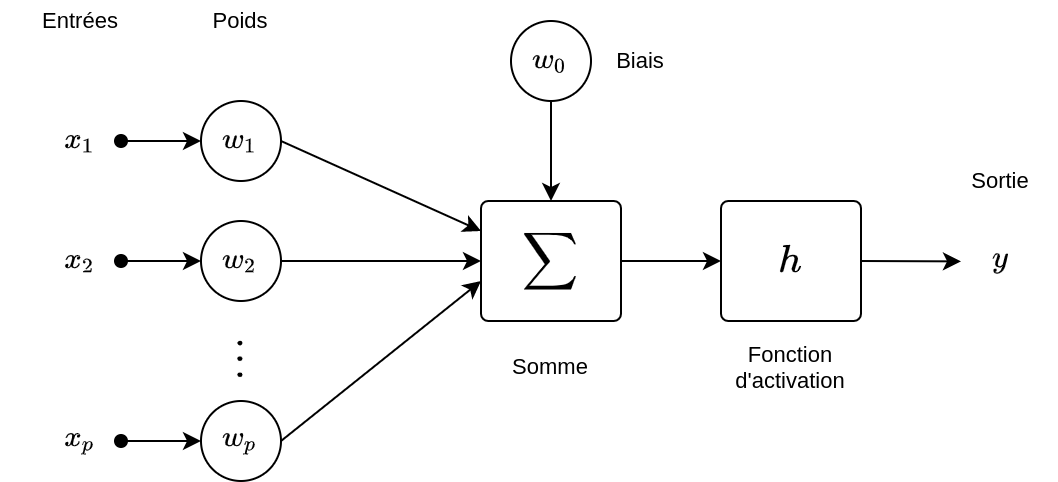
\includegraphics[scale=0.30]{Figures/neurone_formel_representation.png}
    \caption{Perceptron de $p$ entrées \cite{noauthor_perceptron_3png_nodate}.}
    \label{fig:neurone_formel}
\end{figure}

\pagebreak

Un perceptron peut également proposer plusieurs sorties. Pour cela, le vecteur de poids augmente ses dimensions aux nombres de sorties et le biais devient un vecteur. Toutes les entrées vont donc être connectées à ces sorties, et multipliées par les poids correspondants. La figure \ref{fig:perceptron_multi_output} illustre la composition d'un perceptron possédant deux sorties. 

\begin{figure}[hbt!]
    \centering
    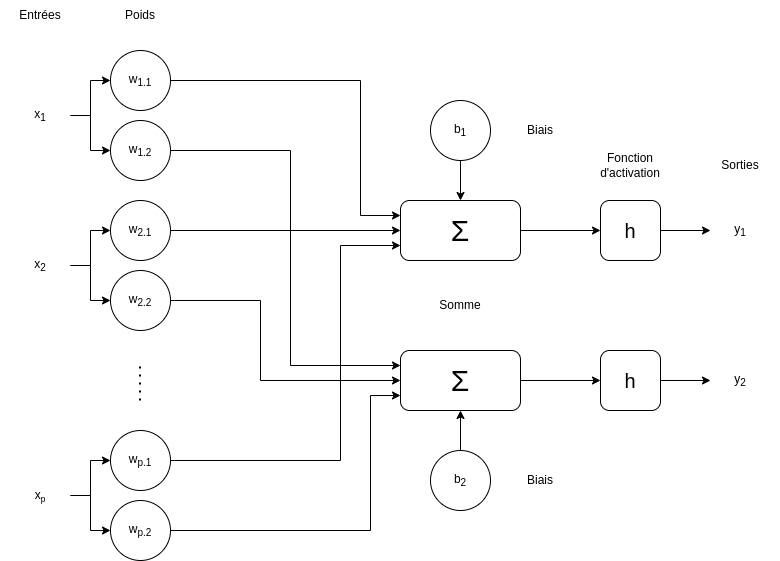
\includegraphics[scale=0.50]{Figures/perceptron_multi_sortie.png}
    \caption{Perceptron de $p$ entrées avec deux sorties.}
    \label{fig:perceptron_multi_output}
\end{figure}

Cette structure relativement simple peut être complexifiée en ajoutant des couches entre l'entrée et la sortie. Une couche correspond à une structure définie, dans notre cas à un autre perceptron. Il s'agit alors d'un perceptron multicouche, un type de réseau de neurones. Celui-ci est caractérisé par le fait qu'il possède une couche d'entrée, au moins une couche cachée, et une couche de sortie. Sur la figure \ref{fig:perceptron_multicouche}, nous pouvons voir comment est composé un perceptron multicouche entièrement connecté. Il est nommé ainsi, car chaque neurone d'une couche est connecté à tous les neurones de la couche suivante.

\begin{figure}[hbt!]
    \centering
    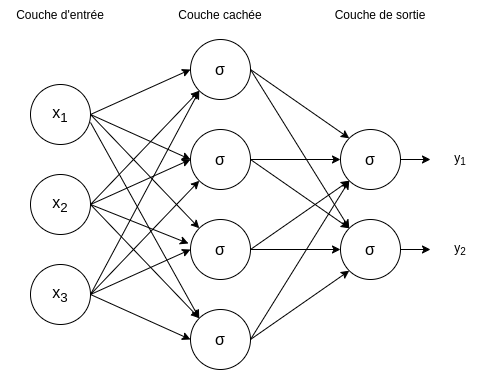
\includegraphics[scale=0.50]{Figures/perceptron_multicouche.png}
    \caption{Perceptron multicouche.}
    \label{fig:perceptron_multicouche}
\end{figure}

\subsection{Apprentissage}

Comme nous avons vu précédemment, un modèle est capable d'effectuer des tâches données, comme une classification binaire, lorsqu'il possède les poids et biais adéquats. Dans le cadre du machine learning, ces derniers ne sont pas connus par avance, et varient en fonction du problème. Il est donc nécessaire que le modèle passe par une phase d'apprentissage ou celui-ci va s'entraîner afin de définir les paramètres les plus adaptés. Ce sont donc ceux-ci qui vont évoluer jusqu'à ce qu'ils permettent d'obtenir, si cela est possible, la/les sorties escomptées \cite{fleuret_deep_nodate-3}.

Il existe différents types d'apprentissages, cependant, dans le cadre de ce travail, nous allons aborder le cas de l'apprentissage supervisé qui correspond à notre cas. En effet, ce type d'apprentissage est défini par des classes prédéterminées et des exemples connus qui sont étiquetés.

L'entraînement du modèle se divise en deux parties. La première consiste à effectuer toutes les opérations définies par notre réseau de neurones sur les entrées d'entraînement. Ces entrées sont divisées en lots, ou "batchs" en anglais, qui définissent le nombre d'échantillons avec lesquels le modèle va travailler avant de mettre à jour les paramètres. Cette phase est communément appelée "forward pass" ou propagation avant en français.

La deuxième va réaliser l'inverse, c'est-à-dire une propagation arrière "backward pass". Le but de cette partie est de rétropropager l'erreur depuis la sortie vers l'entrée, et de mettre à jour les paramètres du modèle, grâce un algorithme d'optimisation, afin de minimiser l'erreur lors des prochaines itérations.

L'erreur utilisée par la backward pass est calculée en évaluant le résultat en sortie du modèle avec la sortie attendue. Cette évaluation est réalisée grâce à une fonction de coût qui varie suivant le problème à traiter. Dans ce travail par exemple, la fonction coût \acrfull{mse} est utilisée. Celle-ci est définie comme suit :

\[\acrshort{mse}=\frac{1}{n}\sum^{n}_{i=1} (Y_i-\hat{Y}_i)^{2}\]

Où $n$ est le nombre de prédictions, $Y$ est le vecteur correspondant aux valeurs à prédire, $\hat{Y}$ est le vecteur contenant les valeurs prédites. Comme le nom de cette fonction le laisse deviner, celle-ci calcule la moyenne de l'erreur au carré, pour laquelle l'erreur correspond simplement à la différence entre la valeur à prédire et la valeur prédite.

Lors de la rétropropagation de l'erreur, il est nécessaire de mettre à jour les paramètres. Pour ce faire, il faut utiliser un algorithme d'optimisation. Il en existe plusieurs, néanmoins, nous allons nous baser sur la descente de gradient pour les explications à suivre. En effet, ce dernier est très connu, et permet de trouver un minimum local en allant, à chaque itération, dans la direction opposée au gradient de la fonction à partir du point courant.

Afin de modifier les paramètres de sorte qu'ils minimisent l'erreur, nous devons donc calculer leur gradient. Pour trouver celui-ci, il faut calculer la dérivée de la fonction de coût par rapport aux paramètres. La mise à jour de la valeur des poids, représentés ici par $w^{(l)}$, est formellement décrite par la formule :

\[w^{(l)}=w^{(l)}-\eta{}\frac{\partial{}\ell}{\partial{}w^{(l)}}\]

Et pour les biais représentés par $b^{(l)}$ :

\[b^{(l)}=b^{(l)}-\eta{}\frac{\partial{}\ell}{\partial{}b^{(l)}}\]

Dans ces formules, nous pouvons voir apparaître le symbole $\eta$ qui correspond au taux d'apprentissage. Celui-ci a un impact direct sur l'apprentissage. En effet, lorsque $\eta$ est élevé la valeur des paramètres sera également modifiée par une valeur plus importante. Cela implique, notamment au début de l'entraînement, que les paramètres vont rapidement converger vers la solution minimisant la fonction de coût. Or, à partir d'un moment, si $\eta$ est trop élevé, la valeur des paramètres va osciller autour de la solution minimisant la fonction de coût sans pouvoir l'atteindre. Inversement, lorsque $\eta$ est faible, il faudra plus de temps aux paramètres pour converger vers la solution minimisant la fonction de coût, sans parler du risque de rester piéger dans un minimum local. Nous pouvons observer ces principes sur la figure \ref{fig:learning_rate_choice}.

\begin{figure}[hbt!]
    \centering
    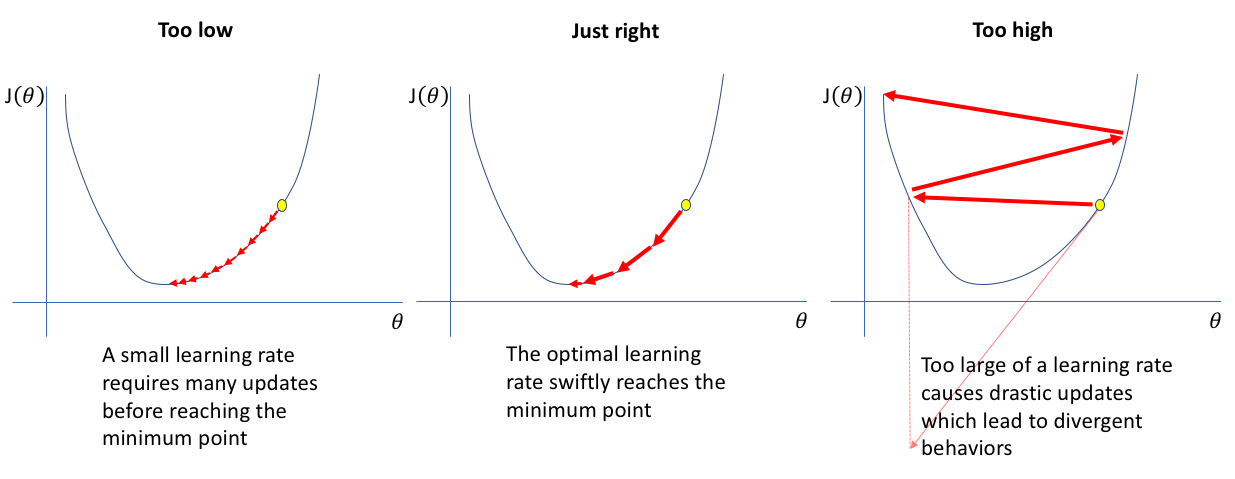
\includegraphics[scale=0.3]{Figures/learning_rate_choice.png}
    \caption{Impact du taux d'apprentissage sur l'entraînement \cite{noauthor_learning_rate_choicepng_nodate}.}
    \label{fig:learning_rate_choice}
\end{figure}

Comme nous avons pu le voir, lors de l'entraînement le modèle va mettre à jour ses poids après chaque batchs. Lorsque celui-ci a parcouru tous les batchs contenant l'ensemble des données d'entraînement, le réseau de neurones vient de réaliser une époque (epoch en anglais). Cependant, même si le jeu de données prévu est conséquent, il est nécessaire que le modèle itère sur plusieurs époques afin d'être bien entraîné. Ce nombre n'est pas connu à l'avance. S'il est trop faible, le réseau de neurones risque de ne pas bien performer et ne pourra pas généraliser ce qu'il a appris à de nouvelles entrées. Ce phénomène est appelé sous-apprentissage (underfitting en anglais).

Inversement, si le nombre d'époques est trop élevé, le modèle sera trop entraîné sur les données d'entraînement ce qui aura pour effet d'obtenir d'excellentes performances sur l'ensemble d'entraînement, mais le réseau de neurones ne sera pas capable de généraliser. Le modèle obtiendra donc de pauvres performances sur de nouvelles entrées. Ce fait se nomme surapprentissage (overfitting en anglais).

C'est pour les deux raisons précédentes qu'il est nécessaire de visualiser l'évolution de l'erreur tout au long de l'entraînement pour les données d'entraînement et de validation. Il également important de tester les performances de notre modèle sur un jeu de données qui n'est pas utilisé. Cela nous donne des informations cruciales sur l'évolution de notre réseau de neurones. Nous pouvons par exemple voir ; lorsque l'erreur ne diminue plus, lorsque l'erreur des données de validation augmente alors que celle des données d'entraînement diminue, mais également lorsque le modèle commence à performer moins bien sur notre jeu de données de test. Avec ces indications, il est possible d'estimer le nombre d'époques nécessaires à notre modèle pour qu'il soit suffisamment entraîné pour généraliser sur de nouvelles entrées avec les performances recherchées, sans qu'il ait atteint le problème du surapprentissage.

\subsection{Réseau neuronal convolutif et convolution}

Les réseaux neuronaux convolutifs (\acrshort{cnn}) sont un type d'architecture de réseau de neurones utilisés notamment dans le domaine du traitement d'images \cite{fleuret_deep_nodate-1}. À la différence du perceptron multi-couche qui possède des couches de neurones entièrement connectées, les \acrshort{cnn} utilisent des couches de convolution avec des filtres adaptables qui leur permettent de capturer des motifs locaux tout en préservant leurs relations spatiales, et d'apprendre les caractéristiques de l'entrée. C'est à ce type de réseau de neurones qu'appartiennent les modèles utilisés dans ce travail.\\

L'idée derrière une couche de convolution est qu'elle va appliquer la même transformation linéaire locale à l'ensemble de l'entrée. Ainsi, lorsqu'une transformation est significative à un endroit, elle le sera partout. De plus, la convolution préserve la structure du signal, c'est-à-dire qu'une entrée de dimensions $n$ va conserver ses dimensions en sortie, mais la taille de celle-ci peut changer.

\begin{figure}[hbt!]
    \centering
    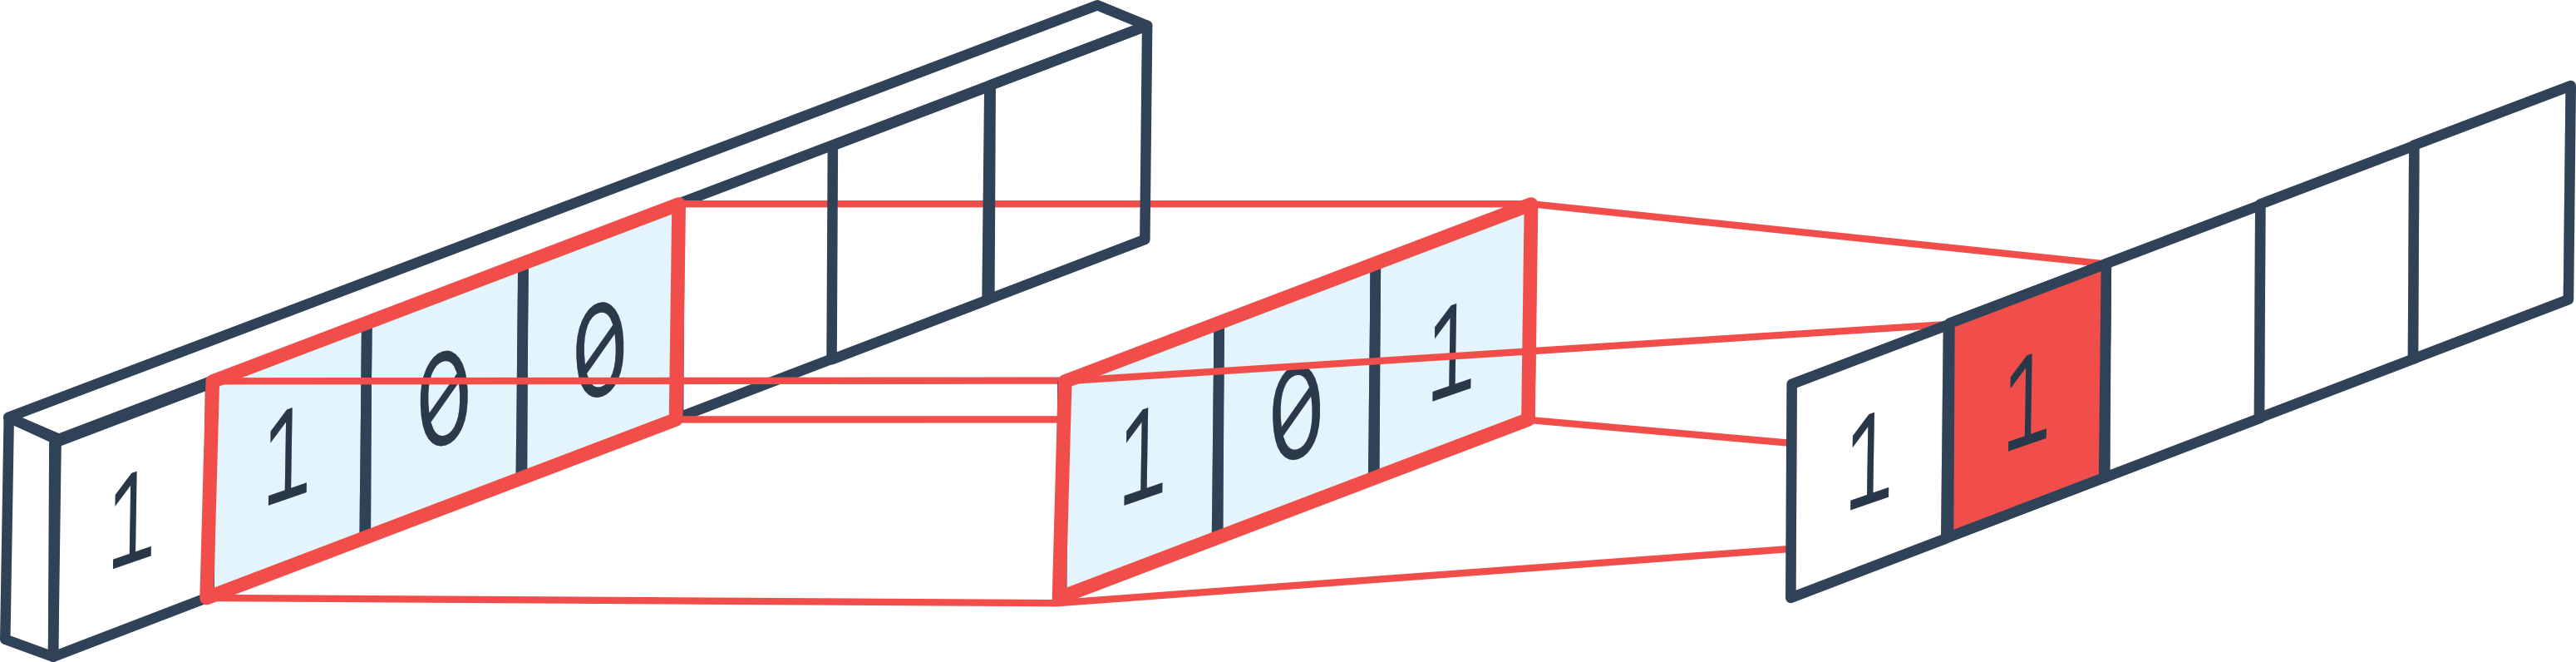
\includegraphics[scale=0.3]{Figures/convolution_exemple.png}
    \caption{Exemple 1D d'une convolution \cite{noauthor_wnixdpng_nodate}.}
    \label{fig:convolution_exemple}
\end{figure}

La convolution consiste, comme nous pouvons le voir sur la figure \ref{fig:convolution_exemple}, en un noyau de convolution, qui correspond à un vecteur de poids (aussi appelé kernel ou filtre), et qui réalise un produit scalaire sur une partie de même taille du signal en entrée. Tout comme il est possible de l'observer sur la figure \ref{fig:convolution_stride_example}, le kernel va traverser l'ensemble du signal à un pas donné qui est nommé stride.

\begin{figure}[hbt!]
    \centering
    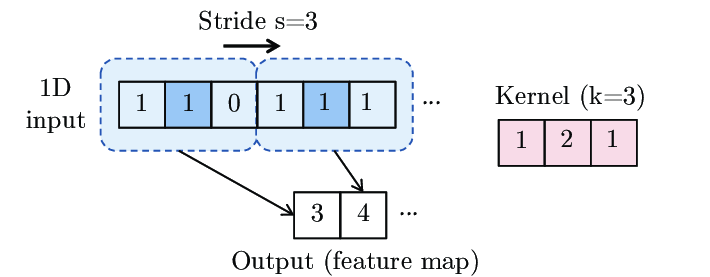
\includegraphics[scale=1.2]{Figures/convolution_stride_example.png}
    \caption{Exemple de stride sur une entrée à une dimension \cite{noauthor_figure_nodate}.}
    \label{fig:convolution_stride_example}
\end{figure}

Par défaut, le stride est de $1$, cependant, lorsque celui-ci est supérieur à $1$, il est possible que le noyau ne puisse pas couvrir l'ensemble de l'entrée et que certaines valeurs se retrouvent ignorées. Pour une entrée $x$ à une dimension de longueur $m$ et pour un kernel $w$ à une dimension de longueur $n$, la convolution au point $i$ (avec un stride de un) peut être formellement décrite comme :

\[
(x * w)_i = \sum^{n}_{j=0} x_{i+j} \cdot w_j
\]

Ce procédé implique que la sortie de notre convolution, bien que de même dimension, n'aura pas la même taille que l'entrée. Celle-ci peut être calculée à partir de la taille de l'entrée et celle de la convolution qui va être appliquée. Par exemple, dans le cas d'une image, l'entrée sera de taille $C \times H \times W$, où $C$ correspond au nombre de canaux (généralement trois, pour $RGB$), $H$ et $W$ respectivement à la hauteur et largeur. La couche de convolution aura un paramètre $D$ correspondant au nombre de kernels qui seront appliqués, et chacun aura une taille définie par $C \times h \times w$, le nombre de canaux est identique à celui de l'image. La sortie d'une telle convolution sera de taille $D \times (H - h + 1) \times (W - w + 1)$. La figure \ref{fig:image_convolution_example} illustre une convolution entre une image $RGB$ de taille $W \times H \times C$ et deux filtres de taille $w \times h \times C$.

\begin{figure}[hbt!]
    \centering
    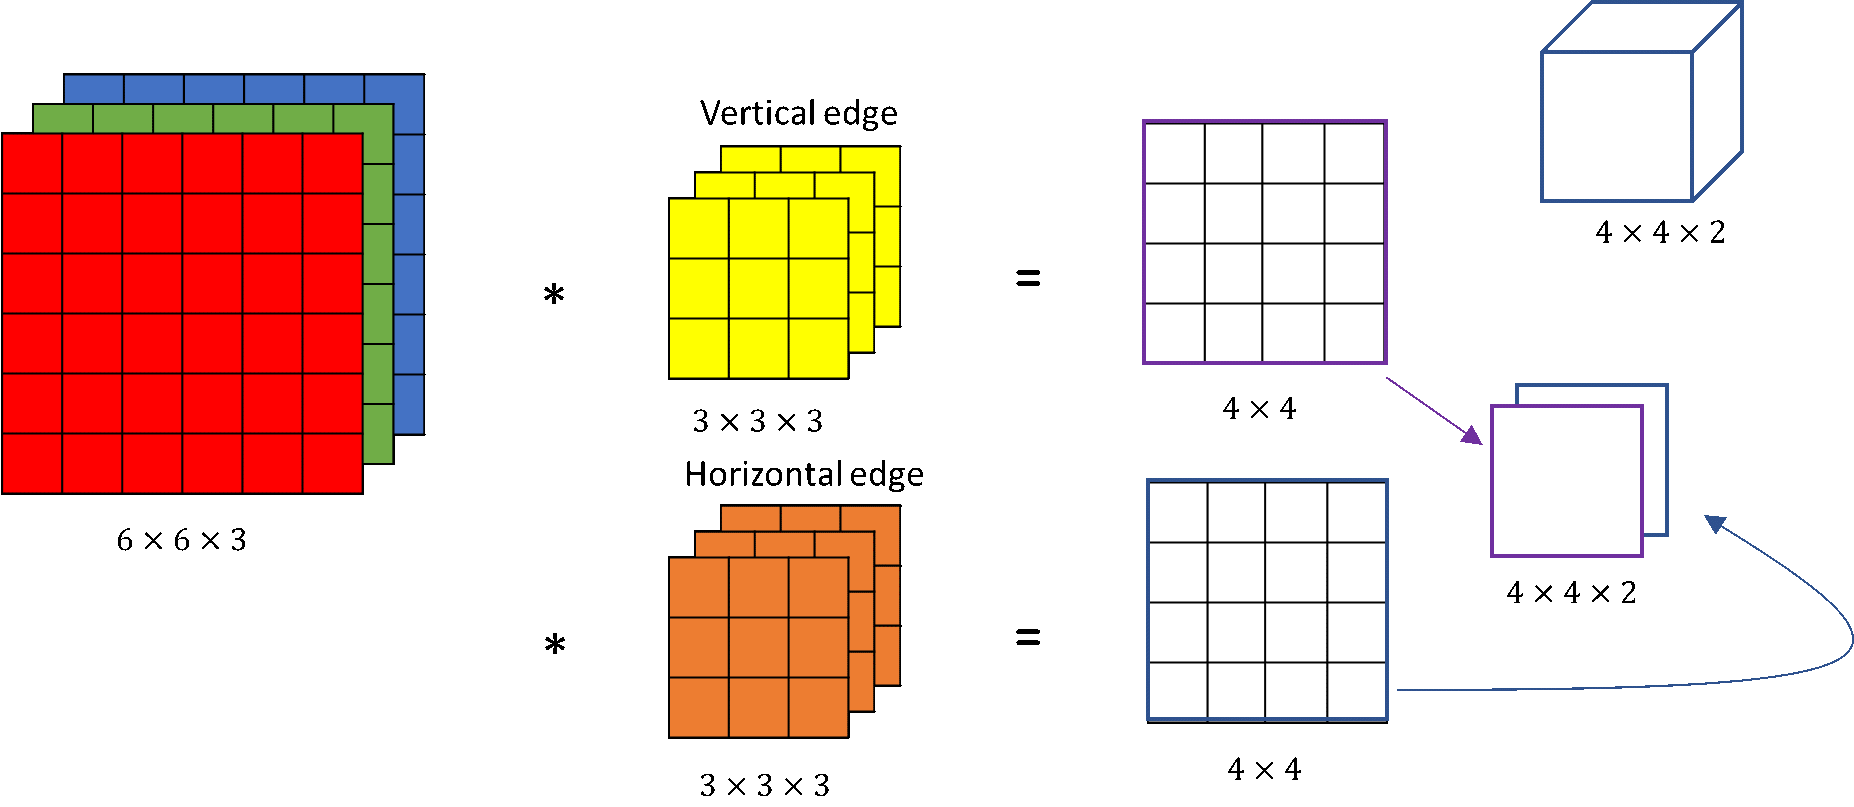
\includegraphics[scale=0.38]{Figures/image_convolution_example.png}
    \caption{Résultat d'une convolution entre une image RGB et deux filtres différents \cite{noauthor_06_09png_nodate}.}
    \label{fig:image_convolution_example}
\end{figure}

Comme vu précédemment, la taille de la sortie d'une convolution est plus petite que celle de l'entrée. Même si cela n'est pas forcément critique, lorsque plusieurs couches de convolutions s'enchaînent, cette différence va s'accroître. Ainsi, pour limiter cet effet, il est possible d'utiliser ce qui est appelé padding. Ce procédé consiste à ajouter des zéros autour de notre entrée avant d'appliquer la convolution afin de gérer la taille de la sortie. La figure \ref{fig:convolution_padding_example} montre un exemple de padding autour d'une entrée à deux dimensions.

\begin{figure}[hbt!]
    \centering
    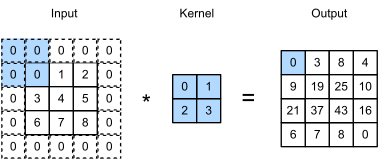
\includegraphics[scale=0.6]{Figures/convolution_padding_example.png}
    \caption{Exemple de convolution avec padding \cite{mohammed_spatiotemporal_2024} Figure 1.}
    \label{fig:convolution_padding_example}
\end{figure}

\subsection{Fonctions d'activation}
\label{sec:fa}

Comme nous avons pu le voir dans la section sur le \hyperref[sec:perceptron]{perceptron}, les fonctions d'activation font partie intégrante de la structure d'un réseau de neurones. Celles-ci sont généralement des fonctions non linéaires appliquées à la sortie d'un neurone.

Nous allons voir les différentes fonctions d'activation qui sont abordées ou utilisées dans ce travail.

Commençons par la fonction \acrfull{relu}. Celle-ci est très simple et définie par :

\[f(x)=max(0,x)\]

Et représentée visuellement par la figure \ref{fig:activation_functions_relu}.

\begin{figure}[hbt!]
    \centering
    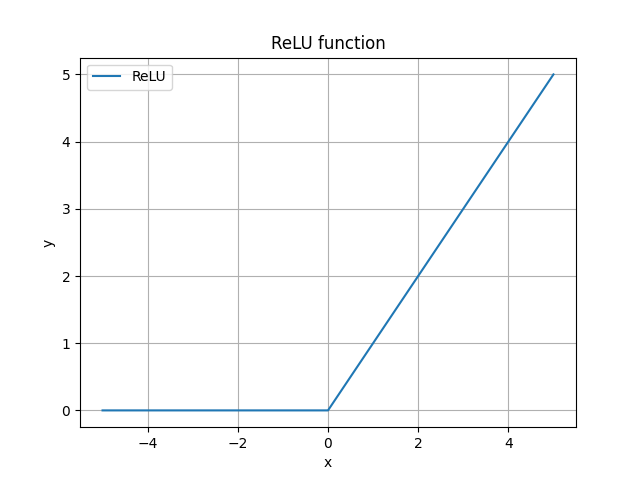
\includegraphics[scale=0.6]{Figures/activation_functions/relu.png}
    \caption{Fonction d'activation \acrshort{relu}.}
    \label{fig:activation_functions_relu}
\end{figure}

La deuxième fonction utilisée est la sigmoïde. Celle-ci est plus complexe que la \acrshort{relu}, et décrit une courbe en forme de S comme visible sur la figure \ref{fig:activation_functions_sigmoid}. Les résultats de cette fonction sont contenus dans l'intervalle $[0;1]$. Cela permet d'obtenir des valeurs similaires à des probabilités qui sont notamment utilisées dans le modèle Resnet18+Tête, décrit dans la section \ref{sec:resnet18}, pour établir le score de confiance de la prédiction réalisée par le neurone. Voici la formule la décrivant :

\[f(x)=\frac{1}{1+e^{-x}}\]

\begin{figure}[hbt!]
    \centering
    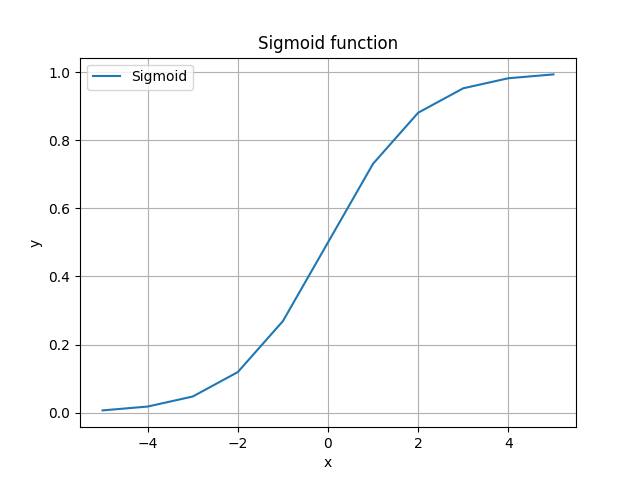
\includegraphics[scale=0.6]{Figures/activation_functions/sigmoid.png}
    \caption{Fonction d'activation sigmoïde.}
    \label{fig:activation_functions_sigmoid}
\end{figure}

La fonction \acrfull{silu} est tout comme la fonction \acrshort{relu} un redresseur. Il s'agit d'une variante qui évite que sa dérivée devienne nulle lorsque la valeur en entrée est négative. Comme il est possible de le voir sur la figure \ref{fig:activation_functions_silu} les valeurs négatives, bien que plus petites, sont toujours présentes. Cette fonction est définie par :

\[f(x)=x \cdot sigmoid(x)\]

\begin{figure}[hbt!]
    \centering
    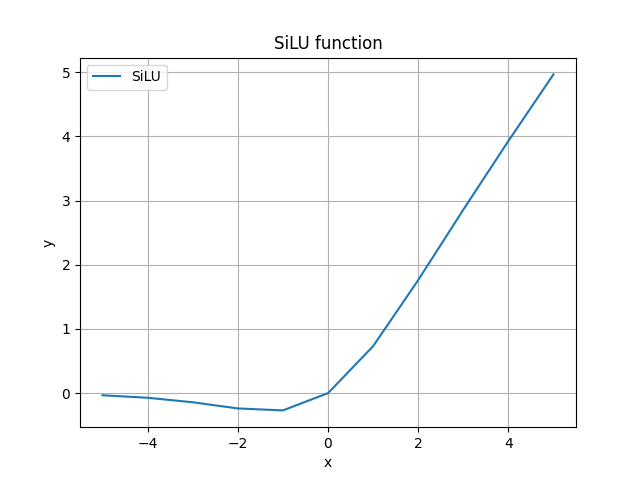
\includegraphics[scale=0.6]{Figures/activation_functions/silu.png}
    \caption{Fonction d'activation sigmoïde.}
    \label{fig:activation_functions_silu}
\end{figure}

Finalement, la fonction swish ressemble à la fonction \acrshort{silu}, à la différence qu'elle possède un paramètre $\beta$. Lorsque ce dernier est défini à 1 alors les deux fonctions sont identiques. Dans la bibliothèque Keras qui a été utilisée, la fonction swish est équivalente à la fonction \acrshort{silu}.
\newpage

\subsection{Fonction de pooling}

Le pooling est un concept important des réseaux de neurones convolutifs. Il s'agit d'une opération qui permet de diminuer la taille de l'entrée tout en préservant les caractéristiques de cette dernière \cite{fleuret_deep_nodate}. Cela permet ainsi de réduire la quantité de paramètres nécessaires dans le réseau, et par extension le nombre de calculs.

Il existe différentes fonctions de pooling, néanmoins nous allons nous concentrer sur les deux utilisées dans ce travail.

Le max-pooling est une opération de pooling qui va parcourir l'entrée par "fenêtres" d'une taille fixée par avance, et ressortir la valeur maximale de chaque zone pour générer la sortie. Sur l'entrée suivante à une dimension : $[1,2,3,4,3,2]$, pour une fenêtre de taille 3, nous aurons en sortie : $[3,4]$. En effet, nous avons appliqué notre première fenêtre de taille 3 sur l'entrée pour traiter juste la partie : $[1,2,3]$, pour laquelle nous avons retenu uniquement la valeur la plus élevée. Puis de même avec la deuxième partie de l'entrée : $[4,3,2]$.  La figure \ref{fig:maxpool_example} illustre le principe à partir d'une entrée de taille 4x4 à laquelle un max-pooling de 2x2 est appliqué.

\begin{figure}[hbt!]
    \centering
    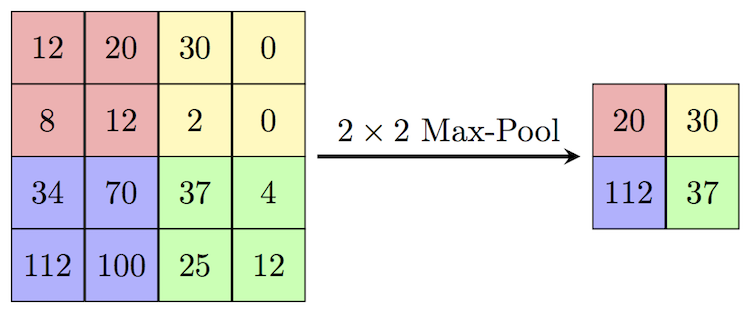
\includegraphics[scale=1.4]{Figures/maxpool_example.png}
    \caption{Exemple d'application de max-pooling 2x2 sur une entrée 4x4 \cite{noauthor_maxpoolsample2png_nodate}.}
    \label{fig:maxpool_example}
\end{figure}

L'average-pooling est une autre fonction de pooling qui s'exécute de la même façon que le max-pooling. Or, cette fois-ci il s'agit de la moyenne des éléments présents dans la fenêtre qui sont calculés.

La taille de la sortie résultant d'une opération de pooling peut être calculée. Supposons une entrée de taille $N \times C \times H \times W$, et un filtre de taille $(h, w)$. L'opération de pooling est appliquée séparément sur chaque canal, et produit la sortie de taille $N \times C \times [H/h] \times [W/w]$.

Par défaut, le pooling utilise un padding de zéro et un stride égal à la taille du filtre. 

\subsection{Normalisation par lots}
\label{subsec:batch_norm}

La normalisation par lots (batch normalization) est un procédé visant à accélérer et stabiliser l'entraînement des réseaux de neurones, ce qui peut améliorer leurs performances. Succinctement, son objectif est de maintenir des statistiques d'activations correctes, afin d'éviter qu'une couche doive s'adapter aux changements d'activations de la couche précédente en plus de ses propres changements. 

Pendant l'entraînement, la normalisation par lots ajuste et redimensionne les valeurs d'entrée en fonction de la moyenne et de la variance calculée dans le lot en cours. Lors des tests, elle utilise les moments empiriques estimés pendant la phase d'entraînement.

\subsection{Sauts de connexions}
\label{subsec:skip_connections}

Les sauts de connexion sont un type de raccourci qui relient la sortie d'une couche à une entrée qui n'est pas à la suite de cette dite couche. Ceux-ci sont notamment utilisés dans les réseaux neuronaux résiduels, mais également dans d'autres types d'architecture. Le principe est très simple, il s'agit d'une connexion qui crée un nouveau chemin qui saute un nombre défini de couches, puis qui va à s'insérer à l'entrée d'une autre couche soit par concaténation, addition, multiplication, etc..

La figure \ref{fig:skip_connections} illustre très bien ce principe. L'entrée du bloc A est à la fois passée dans le bloc A, et additionnée avec la sortie de ce même bloc et plus loin même additionné avec l'entrée et la sortie du bloc C.

\begin{figure}[hbt!]
    \centering
    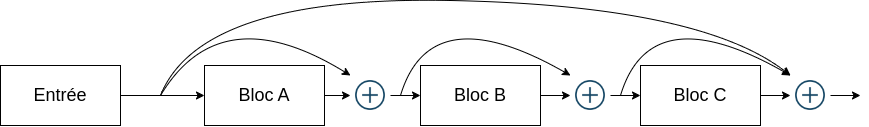
\includegraphics[scale=0.45]{Figures/skip_connections.png}
    \caption{Exemple de sauts de connexions.}
    \label{fig:skip_connections}
\end{figure}

L'utilisation des sauts de connexions permet de diminuer l'effet de la disparition du gradient. Ce fléau se produit lorsque le gradient est très petit. Comme la mise à jour des poids utilise une valeur proportionnelle à la dérivée de l'erreur par rapport au poids en question, celui-ci tend à disparaître pouvant provoquer l'arrêt de l'apprentissage.

\newpage

\section{YOLOv8}
\label{sec:yolov8}

Le premier modèle utilisé dans ce travail est un réseau de neurones convolutifs très populaire issu de la famille \acrfull{yolo} nommé YOLOv8. Sa première version publiée en juin 2015 \cite{redmon_you_2016} s'est fait connaître pour sa grande vitesse et ses hautes performances dans la détection et segmentation d'images. Présentés dans son article, \acrshort{yolo} et sa variante Fast YOLO obtiennent respectivement un \acrshort{map} de 63.4 pour 45 images par seconde, et un \acrshort{map} de 52.7 pour 155 images par secondes [table 1], un ratio de performances beaucoup plus élevé que les modèles couramment utilisés à ce moment-là. Cela en a fait un excellent choix pour des applications en temps réel.

Amélioré au fil des années, YOLOv8 est la dernière version développée par Utralytics utilisant les dernières avancées en deep learning et vision par ordinateur, qui propose des performances inégalées en termes de vitesse et de précision \cite{ultralytics_home_nodate}.

\subsection{Description du modèle}

Afin de comprendre comment fonctionne le modèle, reprenons l'implémentation initiale de YOLO mise au point par Joseph Redmon, et Santosh Divvala. Contrairement aux modèles proposés jusqu'alors, qui parcouraient plusieurs fois l'image traitée, \acrshort{yolo} propose une approche différente qui parcourt l'image une seule fois. Le principe est simple, comme illustré sur la figure \ref{fig:the_yolo_detection_system}, l'image en entrée est passée à un réseau neuronal convolutif qui va prédire simultanément de multiples boîtes de délimitations, et leurs probabilités d'appartenance à une classe.

\begin{figure}[hbt!]
    \centering
    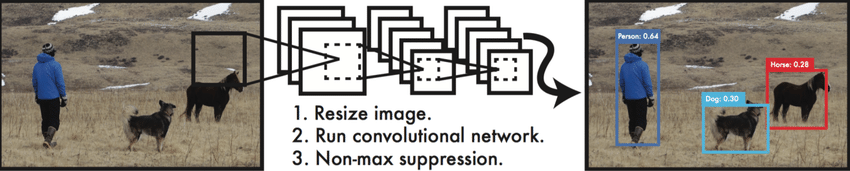
\includegraphics[scale=0.45]{Figures/The-YOLO-Detection-System-17.png}
    \caption{Système de détection de YOLO \cite{noauthor_figure_nodate-1}.}
    \label{fig:the_yolo_detection_system}
\end{figure}

Dans le but de réaliser des prédictions, le réseau de neurones utilise les caractéristiques de toute l'image pour déterminer chaque boîte de délimitation. Le système divise l'entrée en une grille de taille $S \times S$. Si le centre d'un objet se trouve dans une cellule de la grille créée, cette dernière va s'occuper de détecter l'objet. Chaque cellule prédit $B$ boîtes de détection contenant chacunes les éléments suivants : les coordonnées ($x, y$), la longueur, hauteur de l'objet ($w, h$), et le score de confiance. Ce dernier reflète à quel point le modèle est confiant qu'une boîte contienne un objet et l'exactitude de cette prédiction. La confiance est définie formellement par :

\[Confidence = Pr(Object) \cdot IOU^{truth}_{pred}\]

Où nous voyons qu'il s'agit de la probabilité de l'existence d'un objet multiplié par l'intersection sur l'union (voir chapitre \ref{sec:iou}) entre la prédiction et la réalité. Par ailleurs, chaque cellule prédit également la probabilité de chaque classe. Lors de la phase de test, cette valeur est multipliée avec les scores de confiance prédits, ce qui nous retourne le score de confiance de chaque classe donnée pour chaque boîte. Ce score prend en compte la probabilité d'occurrence de la classe donnée dans la boîte et également à quel point la boîte prédit l'objet. La figure \ref{fig:yolo_system_detection_class_and_boxes} illustre ce principe.

\begin{figure}[hbt!]
    \centering
    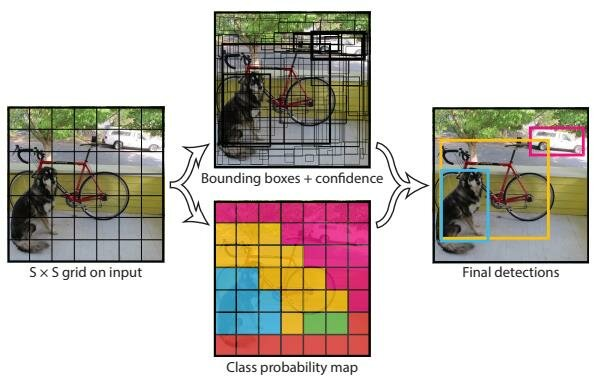
\includegraphics[scale=1.4]{Figures/yolo_system_detection_class_and_boxes.png}
    \caption{Le modèle de YOLO \cite{noauthor_figure_nodate-2}.}
    \label{fig:yolo_system_detection_class_and_boxes}
\end{figure}

Regardons à présent d'un peu plus près l'architecture du réseau représentée sur la figure \ref{fig:yolo_architecture}. Celle-ci contient 24 couches de convolutions suivies par 2 couches complètement connectées qui vont générer une sortie de taille $S \times S \times (B \cdot 5 + C)$ où $S$ correspond à la taille de la grille, $B$ le nombre de boîtes par cellules, et $C$ le nombre de classes.

\begin{figure}[hbt!]
    \centering
    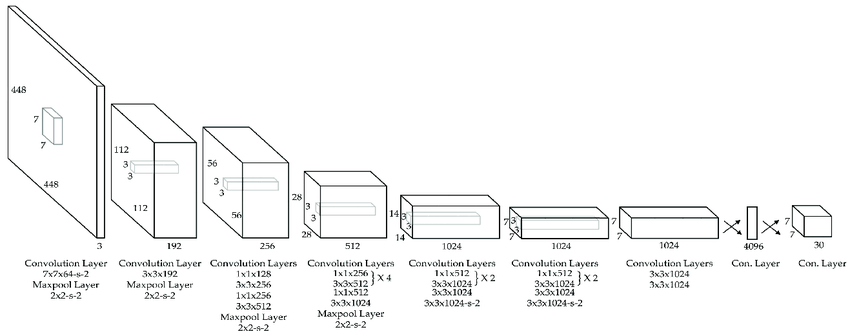
\includegraphics[scale=0.5]{Figures/yolo_architecture.png}
    \caption{Architecture de YOLO \cite{noauthor_figure_nodate-3}.}
    \label{fig:yolo_architecture}
\end{figure}

À présent que le modèle de base a été défini, nous pouvons résumer brièvement l'évolution de celui-ci. En 2016 sort YOLOv2 aussi connut sous le nom de YOLO9000 \cite{redmon_yolo9000_2016}, améliorant YOLO. Cette version conçue pour être plus rapide et précise est aussi capable de détecter une plus grande variété de classes. Ceci est possible grâce à l'utilisation d'un réseau de base appelé Darknet-19 exploitant les avantages de la batch normalization (\ref{subsec:batch_norm}), mais aussi grâce aux boîtes d'ancrage. Celles-ci sont un ensemble de boîtes de délimitations de différents formats et tailles prédéfinies, qui permettent de détecter une plus grande variété d'objets.\\

En 2018 YOLOv3 est publié \cite{redmon_yolov3_2018}. Celui-ci utilise une version améliorée du réseau de base appelé Darknet-53. YOLOv3 améliore également l'utilisation des boîtes d'ancrages en leur permettant de modifier leur échelle et leur octroyant une plus grande variété de formats pour correspondre au mieux aux objets détectés. Finalement, ce modèle introduit le concept de \acrfull{spp}, qui expliqué simplement permet de se débarrasser de la contrainte d'utiliser une image de taille fixe.\\

YOLOv4 introduit en 2020 \cite{bochkovskiy_yolov4_2020} utilise une nouvelle architecture nommée CSPDarknet53, une variante de l'architecture ResNet conçue pour la détection d'objet. Il est le premier à décomposer le modèle en plusieurs parties (modèle de base, cou, et tête). Il garde la même tête de détection utilisée par YOLOv3, mais modifie la génération des boîtes d'ancrages.\\

Apparu également en 2020 YOLOv5 \cite{jocher_yolov5_2020} possède un nouveau réseau de base plus complexe appelé EfficientDet. Il réutilise les principes des précédents modèles tout en les améliorant. Cela lui permet d'obtenir de meilleures performances et une meilleure généralisation à un plus grand ensemble de classes.\\

En 2022 deux versions de YOLO sortent à quelques mois d'intervalle, la v6 \cite{li_yolov6_2022} et la v7 \cite{wang_yolov7_2022}. Les deux proposent leurs propres améliorations vis-à-vis de leurs prédécesseurs que nous n'aborderons pas dans ce travail. YOLOv6 a été pensé pour être utilisé dans l'industrie, et YOLOv7 à sa sortie a surpassé tous les détecteurs d'objets en termes de vitesse et de précision.\\

Finalement en janvier 2023, la dernière version de YOLO développé par Utralytics sort. Lors de l'écriture de ce rapport, YOLOv8 n'a pas encore d'article dédié \cite{jocher_ultralytics_2023}. 

YOLOv8 propose cinq versions de tailles différentes, permettant de facilement choisir une version du modèle en fonction de ses besoins. La différence réside dans le nombre de filtres utilisés par les convolutions, et la profondeur du module C2f. Le modèle est capable de réaliser différentes tâches de vision par ordinateur telles que : la détection d'objet, la segmentation, l'estimation de pose, le suivi, et la classification. Son architecture décrite par la figure \ref{fig:yolov8_architecture} est composée de plusieurs éléments clefs. Il contient un réseau de base similaire à celui de YOLOv5, une couche de \acrfull{sppf}, un module C2f, et un module de détection. Le réseau de base s'occupe d'extraire les caractéristiques principales de l'entrée, puis cette sortie est passée à la couche \acrshort{sppf} qui à l'aide des couches de convolutions la suivant, vont traiter les caractéristiques à différentes échelles. Le module C2f est l'amélioration d'un module déjà existant en YOLOv5 et permet de se passer de la partie "cou" de l'architecture. Il s'agit d'une version accélérée du Cross Stage Partial Bottleneck utilisant deux convolutions, qui a pour but de concaténer les caractéristiques principales à de l'information contextuelle afin d'améliorer la précision de la détection. Finalement, le module de détection utilise un modèle sans ancrage avec une tête découplée afin d'exécuter indépendamment les tâches de classification, régression, ou encore de détection d'objet. Concernant le modèle sans ancrages, celui-ci utilise également un système de grille comme pour les boîtes à ancrages. La différence réside dans le fait que lorsqu'un objet est détecté dans une cellule, la première va estimer l'écart du centre de l'objet à partir du centre de la cellule, mais aussi sa hauteur et largeur. La deuxième va quant a elle estimer l'écart de l'objet détecté par rapport à des ancres prédéfinies.

\begin{figure}[hbt!]
    \centering
    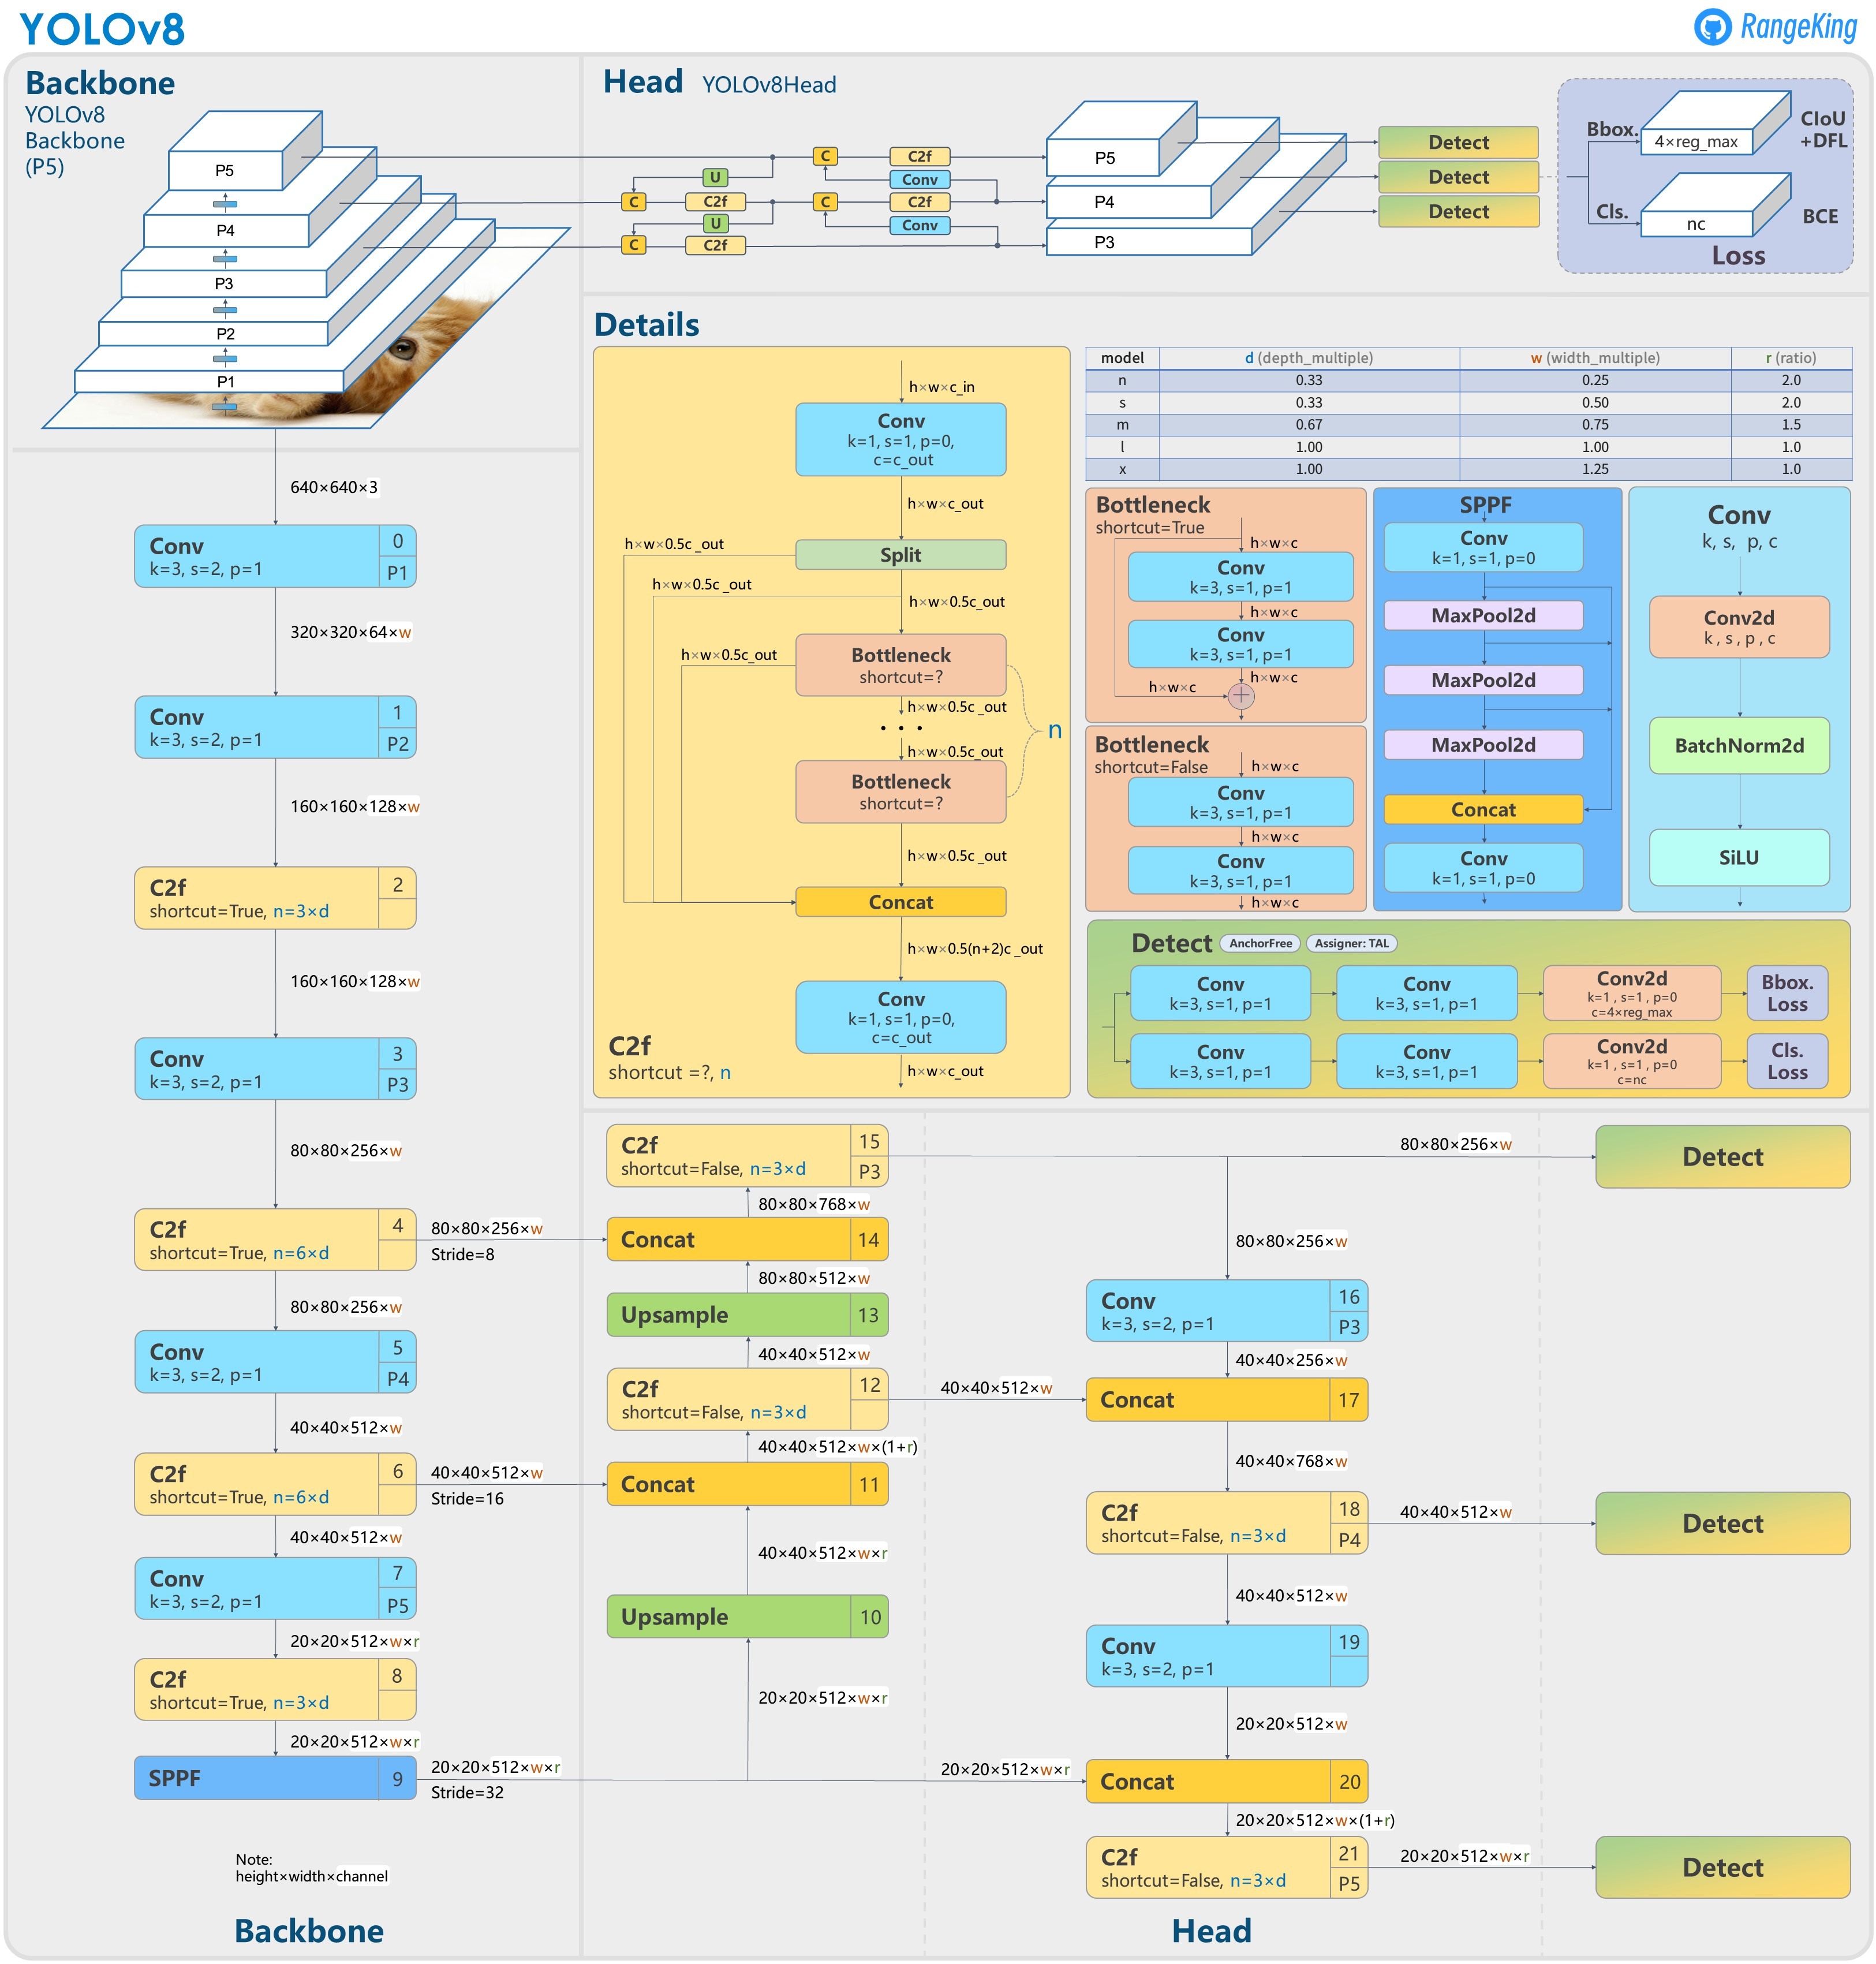
\includegraphics[scale=0.17]{Figures/yolov8_architecture.jpg}
    \caption{Architecture de YOLOv8 \cite{noauthor_brief_nodate}.}
    \label{fig:yolov8_architecture}
\end{figure}

\subsection{Utilisation du modèle}
\label{subsec:yolov8_utilization}

La version de YOLOv8 proposée par Ultralytics a été développée à l'aide de la bibliothèque Pytorch sur Python. Étant donné que nous souhaitons synthétiser le modèle à l'aide du paquet Python \acrshort{hls4ml} (\ref{HLS4ML}), et que celui-ci ne supporte que partiellement la bibliothèque Pytorch, nous avons réfléchi à deux approches différentes impliquant la bibliothèque Keras qui est supportée, tout en nous laissant l'accès au code pour pouvoir quantifier le code à l'aide de la librairie QKeras.

La première consistait à développer le modèle à partir de zéro. Malgré l'architecture et le code Pytorch à disposition, réaliser une telle implémentation restait un travail trop conséquent. Cependant, même si cette solution n'a pas été retenue, nous avons tout de même pu contribuer à la correction de l'architecture publiée.\\

La deuxième approche, qui est celle retenue, consiste à reprendre la librairie KerasCV \cite{noauthor_kerascv_2023} contenant leur propre implémentation en Keras du modèle YOLOv8. Cette solution nous permet de nous concentrer sur l'utilisation pure du modèle tout en nous donnant l'accès complet à leur code pour le modifier comme souhaité.\\

Afin de travailler librement sur le code de KerasCV nous avons forké et modifié leur code tout en développant nos propres scripts. Pour commencer, nous avons réalisé une légère modification dans le code source. Celle-ci concerne la constante \verb|BOX_REGRESSION_CHANNELS| qui est initialisée à 64. Même si elle ne possède pas le même nom que sur l'architecture de YOLOv8, cette dernière est utilisée comme la variable \verb|reg_max| qui correspond à la plage maximale des paramètres des boîtes d'ancrages \cite{noauthor_what_nodate}. Nos images en entrée étant déjà petites, $49 \times 64$, le rayon des jets présents dans celles-ci l'est encore plus et est égales à $4$ pixels. Finalement, nous trouvons empiriquement que la valeur 16 est celle qui donne les meilleurs résultats.\\

Avec notre modèle fonctionnel, nous avons pu réaliser plusieurs entraînements, et tester les prédictions de celui-ci. Lorsque YOLOv8 effectue une prédiction, celui-ci va nous retourner trois listes. La première nommée "boxes" possède les informations relatives à la boîte concernant la prédiction. Elle contient les coordonnées $(x, y)$ mais également la hauteur et largeur de l'objet. La deuxième nommée "classes", contient la classe à laquelle appartient chaque détection. Puis la troisième nommée "confidence", est constituée du score de confiance du modèle au sujet de la prédiction concernée.\\

Concernant les images à fournir au modèle, comme expliqué par Glenn Jocher \cite{noauthor_image_nodate}, créateur de YOLOv5 et YOLOv8, celui-ci travaille sur des entrées dont la taille est un multiple $32$. Cependant, si cela n'est pas le cas, l'image sera automatiquement redimensionnée pour répondre à cette exigence. Pour éviter toute modification de nos images, nous avons décidé d'augmenter la taille de notre matrice vers le premier multiple de $32$, et obtenons ainsi une nouvelle matrice de $64 \times 64$. L'axe $\phi$ n'est pas modifié étant donné qu'il est déjà égal à cette taille. En revanche, l'axe $\eta$ est augmenté par des indices dont la valeur est définie à $0$.\\

Un point que nous avons constaté en travaillant sur notre modèle est que le nombre de paramètres indiqué sur l'implémentation originale en Pytorch n'est pas identique à celle de Keras. Ainsi, Ultralytics présente le nombre de paramètres suivants en fonction de la taille du modèle comme indiqué sur la table \ref{tab:nb_params_yolov8_pytorch}.

\begin{table}[!ht]
    \caption{Nombre de paramètres pour chaque modèle de YOLOv8 Pytorch}
    \label{tab:nb_params_yolov8_pytorch}
    \rowcolors{2}{gray!25}{white}
    \centering
    \begin{tabular}{ |c||c|  }
        \hline
        \rowcolor{gray!50}
        Modèle & params (M)\\
        \hline
        YOLOv8n & 3.2\\
        YOLOv8s & 11.2\\
        YOLOv8m & 25.9\\
        YOLOv8l & 43.7\\
        YOLOv8xl & 68.2\\
        \hline
    \end{tabular}
\end{table}

Alors que les valeurs des modèles issus de l'implémentation KerasCV correspondent à celles décrites par la table \ref{tab:nb_params_yolov8_kerascv}.

\begin{table}[!ht]
    \caption{Nombre de paramètres pour chaque modèle de YOLOv8 KerasCV}
    \label{tab:nb_params_yolov8_kerascv}
    \rowcolors{2}{gray!25}{white}
    \centering
    \begin{tabular}{ |c||c|  }
        \hline
        \rowcolor{gray!50}
        Modèle & params (M)\\
        \hline
        YOLOv8xs reduced 16x & 0.025779\\
        YOLOv8xs reduced 8x & 0.0679\\
        YOLOv8xs reduced 4x & 0.225522\\
        YOLOv8xs reduced 2x & 0.834286\\
        YOLOv8xs & 3.225894\\
        YOLOv8s & 12.856342\\
        YOLOv8m & 25.665798\\
        YOLOv8l & 39.401462\\
        YOLOv8xl & 61.535974\\
        \hline
    \end{tabular}
\end{table}

Cette différence peut s'expliquer simplement par le fait qu'il s'agit de deux librairies distinctes dont l'implémentation de chaque couche n'est pas identique. Par ailleurs, les noms des modèles sont légèrement différents, mais ils correspondent à la même logique.\\

Finalement, nous avons tenté de synthétiser la version de YOLOv8 à l'aide de \acrshort{hls4ml}. Nous nous sommes retrouvés bloqués par des limitations d'implémentations du paquet. En effet, KerasCV a imbriqué le modèle de base (backbone) dans le modèle YOLOv8. Or, la version 0.7.1 de \acrshort{hls4ml} n'arrive malheureusement pas à extraire les couches d'un modèle imbriqué. Malgré plusieurs essais pour dérouler cette dernière et prémâcher le travail à \acrshort{hls4ml}, celui-ci n'arrivait pas à comprendre ces couches. Une piste suggérée par Pablo Strasser un collaborateur scientifique à la HEG, était d'exporter le modèle Keras en ONNX, un format ouvert pour représenter les modèles de machine learning. Cependant, \acrshort{hls4ml} ne supportait pas certaines couches de ce format utilisées par YOLOv8. De plus, certaines couches personnalisées définies dans le code de KerasCV ne sont pas prises en charge par \acrshort{hls4ml}, nécessitant le développement de l'implémentation HLS de ces dernières.

Ainsi, comme le modèle ne pouvait pas être synthétisé sans une réécriture profonde du code et pour une question de temps, nous avons décidé de ne pas quantifier le modèle, mais de tout de même tester ses performances sur notre problème. À la fin de notre travail sur ce modèle, nous avons des scripts permettant d'entraîner le modèle, de l'évaluer, de générer des labels ou des images, mais également de visualiser les résultats obtenus sous forme de tableaux ou de graphes à l'aide de diverses métriques.

\subsection{Génération des labels}
\label{subsec:yolov8_labels_generation}

Afin de pouvoir entraîner le modèle à détecter des jets, il a fallu générer les labels des images passées en entrée. Tout comme pour la génération des images, nous avons voulu stocker les labels dans des fichiers .npy pour les avantages qu'ils présentent. Ce format impose cependant une contrainte, il faut que les tableaux stockés soient tous de même taille. Étant donné que le nombre de jets par image n'est pas fixe, nous avons décidé d'ajouter une classe qui nous permet d'étoffer notre tableau si besoin afin d'obtenir des tableaux d'une taille fixe. Cette "nouvelle classe" est notée la classe 0 et possède toujours les mêmes coordonnées, c'est-à-dire en $(x, y)$  $(55, 32)$. Celle-ci correspond à la partie paddée de l'image qui ne contient aucune information. Dans le cas où il s'agit bien d'un jet que nous souhaitons labéliser, il sera noté comme appartenant à la classe 1 et aux coordonnées $\eta \times \phi$ de la matrice où il se trouve.

Un label est donc défini de la manière suivante : $coordonn\acute{e}e \: \eta, \: coordonn\acute{e}e \: \phi, \: H, \: W, \: classe$.\\

Concernant le nombre de labels, nous avons repris la logique des fichiers .h5. Ceux-ci sont également contraints d'indiquer une taille fixe qui a été définie à 30. C'est cette même constante que nous avons réutilisé.

Lors de la génération des labels, nous vérifions que le jet en cours de labélisation soit compris dans un intervalle plus restreint que celui posé de base. En effet, nous souhaitons ne pas prendre en compte les bords de l'image qui sont plus sensibles dans le cadre de la détection, car ces derniers peuvent contenir un jet partiel pouvant être ou non reconnu comme tel. Comme nous connaissons le rayon d'un jet qui est de 0.4, nous allons travaillé dans l'intervalle $\eta \in \mathbb{R} : \eta \in [-2;2]$ et $\phi \in \mathbb{R} : \phi \in [-2.75;2.75]$ afin de ne pas être confrontés à ces cas.

En ce qui concerne la hauteur et la largeur des jets, nous réutilisons la valeur du rayon d'un jet sur les deux axes ce qui nous donne approximativement 4 pixels pour les deux axes. Étant donné que nous réalisons des conversions d'échelles sur des valeurs arrondies, nous voulons nous assurer d'englober la totalité d'un jet. C'est pourquoi nous décidons d'utiliser 5 pixels de rayon.

De par le format d'entrée attendu par le modèle, les labels doivent être décomposés en deux parties de la façon suivante : $coordonn\acute{e}e \: \eta, \: coordonn\acute{e}e \: \phi, \: H, \: W$ et $classe$. Nous allons donc créer deux tableaux contenant ces informations de façons séparées.

\subsection{Evaluation du modèle}
\label{subsec:yolov8_model_evaluation}

Lorsque le modèle a été entrainé, il est crucial de pouvoir l'évaluer. Pour ce faire, nous avons développé un script d'évaluation afin de générer les résultats nécessaires au calcul des différentes métriques utilisées. Pour cela, nous allons nous servir de nos images et labels dédiés pour l'évaluation.

Nous allons tout d'abord sélectionner pour chaque événement, les jets qui sont dans la zone de détection que nous avons précédemment définie. Suite à cette étape, nous allons parcourir les détections de notre modèle en ne prenant en compte que celles qui ont été réalisées pour la classe 1 (correspondant aux jets), et dans l'intervalle $\eta \in \mathbb{R} : \eta \in [-2;2]$ et $\phi \in \mathbb{R} : \phi \in [-2.75;2.75]$.

Finalement, nous utilisons le seuil de confiance assigné à chaque détection pour déterminer lesquelles doivent être prises en considération et qui seront acceptées ou rejetées par la suite à l'aide de l'intersection sur union (\ref{sec:iou}). 

Pour identifier si un jet détecté est correct ou non, nous allons parcourir tous les labels de l'image en testant à chaque fois si leur \acrshort{iou} est supérieur à un seuil fixé en avance.

\newpage

\section{ResNet18 + Tête}
\label{sec:resnet18}

Le deuxième modèle utilisé est un réseau neuronal convolutif personnalisé. Celui-ci utilise comme base ResNet18 auquel une tête a été ajoutée afin de modifier le classifieur en un détecteur. Ainsi, nous pouvons obtenir des coordonnées et un score de confiance en sortie. Ce modèle a été mis en point avec la volonté de proposer une implémentation simple, possédant peu de paramètres, des performances correctes, et qui puisse être synthétisée avec \acrshort{hls4ml}. ResNet18 répondant à ces critères, nous l'avons donc sélectionné.

\subsection{Description du modèle}

Commençons tout d'abord par décrire le modèle de base. ResNet18 est un réseau neuronal résiduel présenté en 2015 par Kaiming He, Xiangyu Zhang, Shaoqing Ren, et Jian Sun \cite{he_deep_2015} qui propose une architecture facilitant l'entraînement de réseaux profonds. Ce type de réseau utilise les sauts de connexion (\ref{subsec:skip_connections}) afin de pouvoir construire des modèles profonds pouvant posséder un plus grand nombre de couches, tout en diminuant le problème de la disparition du gradient.

Dans l'article, les auteurs présentent cinq variantes de 18, 34, 50, 101, et 152 couches. Bien que les modèles plus profonds aient de meilleurs résultats, nous choisissons le réseau de 18 couches, car celui-ci est le plus petit et donc le plus rapide, tout en proposant des performances acceptables. L'architecture de ResNet18 est illustrée à la figure \ref{fig:resnet18_architecture}.

Le modèle prend en entrée dans sa version originale une image de 224x224x3 où 224x224 correspond à la taille de l'image, et le 3 représente les canaux rouge, vert, bleu. L'entrée est passée dans une première couche de convolution possédant un noyau de $(7,7)$, un stride de $(2,2)$, et un padding de $(3,3)$. Une opération de max-pooling, avec une fenêtre de $(3,3)$ et un stride de $(2,2)$, est par la suite appliquée afin de réduire la dimensionnalité de l'image.

La partie principale du réseau est constituée de huit blocs résiduels. Chacun d'entre eux contient deux couches de convolutions d'un noyau de $(3,3)$ ainsi qu'un saut de connexion (représenté par les flèches pleines sur la figure \ref{fig:resnet18_architecture}) entre l'entrée et la sortie du bloc qui est additionné à ce dernier. Le nombre de filtres double tous les 4 blocs dans l'ordre suivant : $64, 128, 256, 512$. Entre deux blocs d'un nombre de filtres différents, le saut de connexion (représenté par les flèches traitillés sur la figure \ref{fig:resnet18_architecture}) est légèrement modifié et passe par une convolution d'un noyau de $(1,1)$, et un stride de $(2,2)$ afin que la sortie soit de même dimension.

La sortie des ces blocs résiduels est passé dans une opération de global average pooling qui va calculer la moyenne de chaque dimension et ainsi obtenir une sortie de taille $(512,)$.

A ce stade le modèle ResNet18 va passer le résultat de la couche précédente dans une couche de neurones pleinement connectés afin de réaliser la classification sur les mille classes présentes sur ImageNet (une base de données d'images labélisées). C'est à cette étape que nous allons retirer cette couche afin d'y ajouter notre tête de détection, représentée à la figure \ref{fig:resnet18+head_architecture}. Celle-ci est composée d'un nombre $n$ de blocs de détection (D.B. pour Detection Block) correspondant à la manière dont l'image a été subdivisée lors de la labélisation (\ref{subsec:resnet18+head_label_generation}). Chaque bloc va ainsi contribuer à la détection d'un objet dans une région spécifique de l'image. La couche Dense avec deux neurones en sortie va prédire les coordonnées $(x,y)$ de l'emplacement d'un jet, et la couche Dense avec un seul neurone en sortie va établir un score de confiance. Ces deux sorties sont concaténées entre elles, avant d'être à leur tour concaténées avec le reste des prédictions.

\begin{figure}[hbt!]
    \centering
    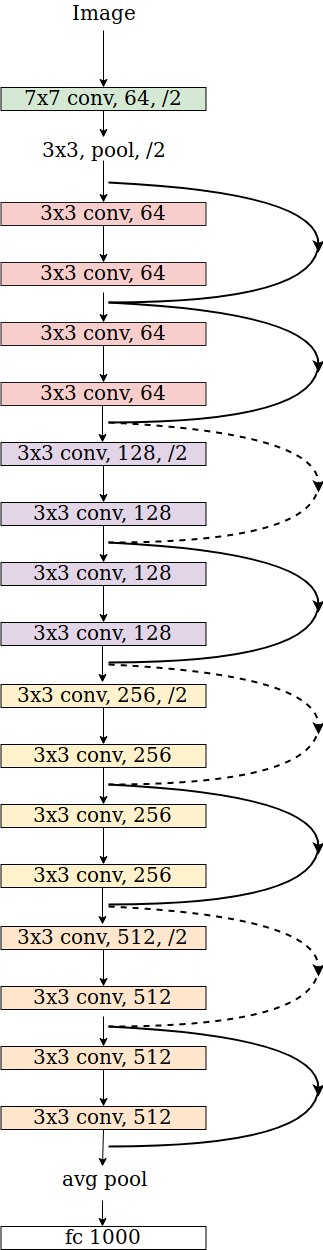
\includegraphics[scale=0.4]{Figures/resnet18_architecture.png}
    \caption{Architecture de ResNet18 \cite{thatsnotmyname71_what_2019}.}
    \label{fig:resnet18_architecture}
\end{figure}

\newpage

\begin{figure}[hbt!]
    \centering
    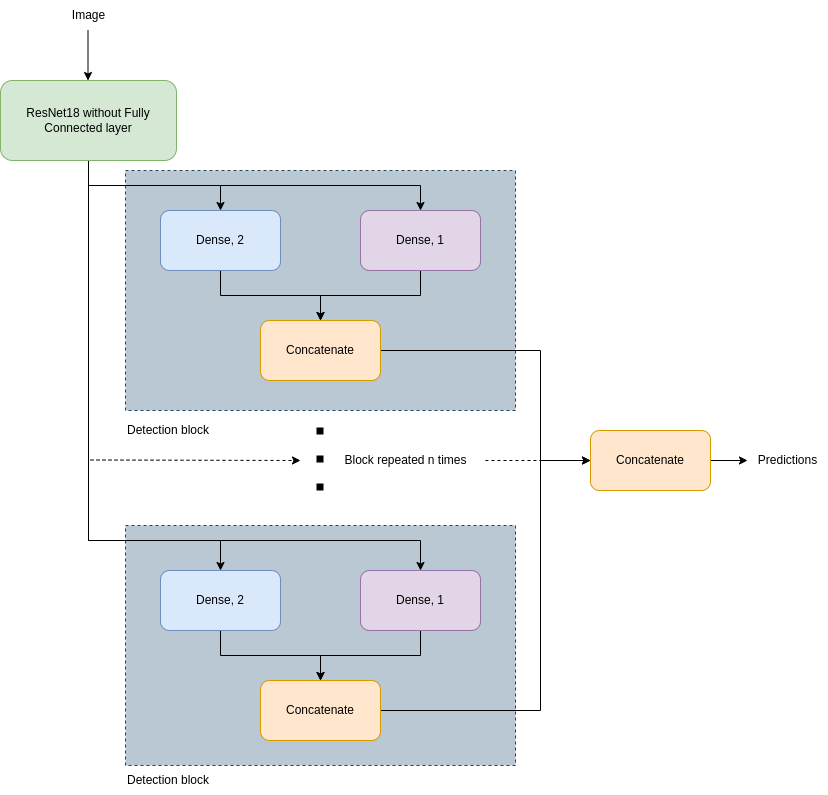
\includegraphics[scale=0.5]{Figures/resnet18+head_architecture.png}
    \caption{Architecture de ResNet18 avec sa tête de détection.}
    \label{fig:resnet18+head_architecture}
\end{figure}

\subsection{Développement de la tête}

Avant d'obtenir la tête utilisée actuellement par notre modèle, nous avons fait plusieurs itérations en les testant à chaque fois. L'idée initiale était d'utiliser un \acrshort{mlp} qui retournerait une sortie similaire à celle de \acrshort{yolo}, c'est-à-dire les coordonnées $(x, y)$, la hauteur et largeur de l'objet, ainsi qu'un score de confidence. Comme nous ne travaillons qu'avec une seule classe, nous avons déjà retiré cette sortie. Nous nous sommes rapidement rendu compte que le modèle peinait à travailler avec la hauteur et largeur des jets. Comme ceux-ci ont toujours le même rayon, nous avons décidé de retirer ces valeurs afin de faciliter l'apprentissage du modèle. Suite à cette étape, nous avons constaté qu'un \acrshort{mlp} plus petit menait à de meilleures performances, jusqu'à ne garder qu'une couche de neurones.

Le neurone générant les coordonnées $(x, y)$ possède un \acrshort{relu} comme fonction d'activation étant donné que nous souhaitons obtenir les coordonnées sur notre matrice. Le neurone générant le score de confiance utilise quant à lui une sigmoïde afin d'obtenir une valeur entre 0 et 1.

\subsection{Utilisation du modèle}

Lors de l'implémentation de notre modèle, nous avons repris la structure de ResNet18 à laquelle nous avons ajouté des blocs de détection en remplacement de la couche de neurones entièrement connectés. De plus, nous avons intégré des couches de normalisation par lots après chaque convolution pour tirer parti de ses avantages.

L'objectif restant le même que pour YOLOv8, nous avons réutilisé les scripts développés précédemment. Nous avons notamment gardé les mêmes images que pour YOLOv8. En effet, la génération des labels étant différente et subdivisant nos images en sous-matrices de taille égales, il était plus pratique de continuer à travailler avec des matrices carrées.

Le modèle retourne en sortie un Tensor avec les prédictions réalisées par chaque bloc de détection sous forme $(x, y, conf)$, où les deux premières valeurs correspondent aux coordonnées et la troisième au score de confiance concernant la présence d'un jet aux indices indiqués.

Concernant la taille du modèle, celle-ci varie en fonction du nombre de blocs de détection et de la taille des filtres de convolution, comme présenté sur la table \ref{tab:nb_params_resnet18+head}. Il est intéressant de noter le nombre de paramètres n'est pas affecté par la quantification du modèle.

\begin{table}[!ht]
    \caption{Nombre de paramètres pour chaque modèle de ResNet18+Tête et différentes tailles de blocs de détections (D.B.)}
    \label{tab:nb_params_resnet18+head}
    \rowcolors{2}{gray!25}{white}
    \centering
    \begin{tabular}{ |c||c|  }
        \hline
        \rowcolor{gray!50}
        Modèle & params (M)\\
        \hline
        (Q)ResNet18+Head 64 D.B. reduced 16x & 0.052008\\
        (Q)ResNet18+Head 64 D.B. reduced 8x & 0.190992\\
        (Q)ResNet18+Head 64 D.B. reduced 4x & 0.730464\\
        (Q)ResNet18+Head 64 D.B. reduced 2x & 2.855424\\
        (Q)ResNet18+Head 64 D.B. & 11.289408\\
        (Q)ResNet18+Head 16 D.B. & 11.215536\\
        (Q)ResNet18+Head 36 D.B. & 11.246316\\
        (Q)ResNet18+Head 121 D.B. & 11.377131\\
        \hline
    \end{tabular}
\end{table}

\subsection{Génération des labels}
\label{subsec:resnet18+head_label_generation}

Tout comme pour la génération des labels avec YOLOv8, nous allons réutiliser le format .npy et la contrainte liée, c'est-à-dire le besoin d'avoir des labels d'une taille fixe entre toutes les images. Par ailleurs, nous conservons la logique d'omettre les jets trop proches des bords de l'image, afin de travailler dans l'intervalle $\eta \in \mathbb{R} : \eta \in [-2;2]$ et $\phi \in \mathbb{R} : \phi \in [-2.75;2.75]$.\\

Contrairement à YOLOv8, l'ordre des labels impacte directement les performances du modèle. La méthode d'annotation choisie est donc cruciale pour obtenir de bons résultats.

Une approche naïve pourrait être d'ordonner la liste des jets d'une image par rapport à l'axe $\eta$ ou $\phi$ et de compléter la taille de cette dernière avec des éléments dans la zone paddée. Bien que cette implémentation soit simple et permette de choisir aisément un nombre arbitraire de neurones, lors de l'apprentissage les premiers neurones seront ceux qui verront un grand nombre de jets. Comme visible sur les figures \ref{fig:visulization_prediction_naive} et \ref{fig:visulization_prediction_naive_mean_std}, le premier neurone réalise des détections sur une grande surface de l'image, puis les neurones suivants réaliseront des détections sur une surface plus petite, jusqu'aux derniers neurones qui ne détecteront plus rien.\\

\begin{figure}[hbt!]
    \centering
    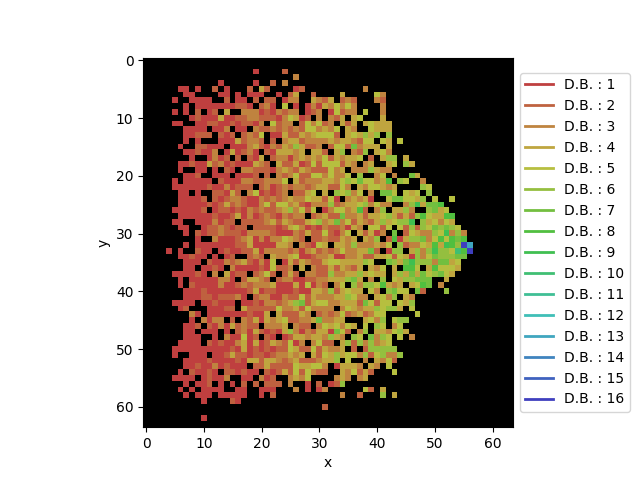
\includegraphics[scale=0.7]{Figures/visulization_prediction_naive.png}
    \caption{Visualisation de l'emplacement des prédictions de chaque bloc de détection du modèle entraîné par la méthode naïve pour le jeu de données "test" avec 16 blocs de détection (D.B.).}
    \label{fig:visulization_prediction_naive}
\end{figure}

\begin{figure}[hbt!]
    \centering
    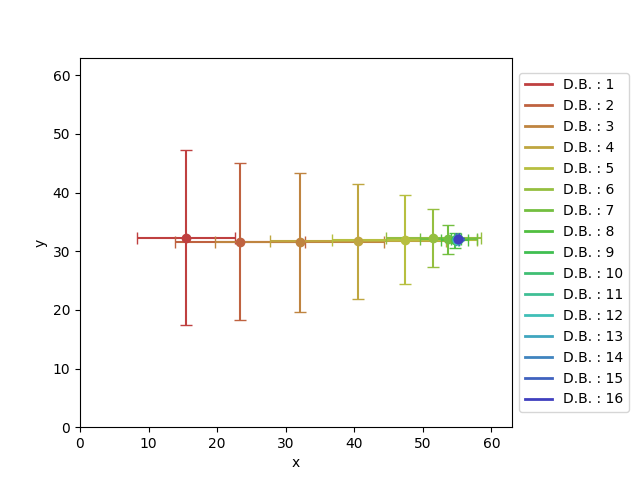
\includegraphics[scale=0.7]{Figures/visulization_prediction_naive_mean_std.png}
    \caption{Visualisation de la moyenne et de l'écart-type des prédictions de chaque bloc de détection du modèle entraîné par la méthode naïve pour le jeu de données "test" avec 16 blocs de détection (D.B.).}
    \label{fig:visulization_prediction_naive_mean_std}
\end{figure}

Une autre approche, qui est celle utilisée, consiste à découper l'image en un nombre de régions prédéterminé. Par exemple, si nous définissons ce nombre de zones à 16 pour notre image de taille $(64 \times 64)$, celle-ci va découper l'image en 16 sous-matrices d'une taille de $(16 \times 16)$. La figure \ref{fig:image_subdivided_like_labels_does} illustre cette application sur une image extraite des données avec en rouge la séparation entre les zones et en blanc le centre de chaque région.

\begin{figure}[hbt!]
    \centering
    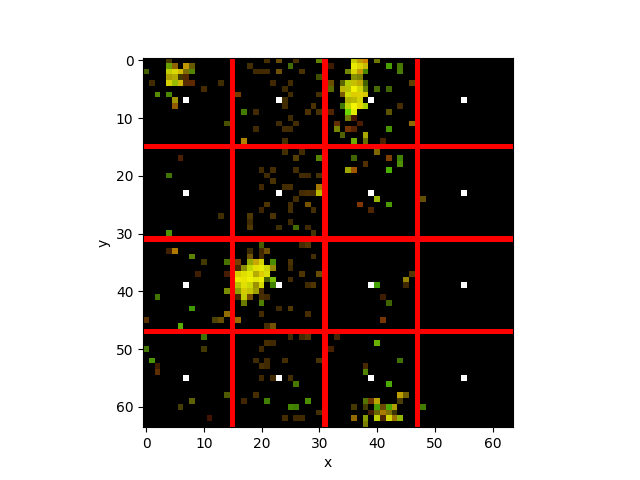
\includegraphics[scale=0.7]{Figures/image_subdivided_like_labels_does.png}
    \caption{Exemple d'image subdivisée en sous partie.}
    \label{fig:image_subdivided_like_labels_does}
\end{figure}

Dans un premier temps, chaque région va s'attribuer le jet le plus proche si celui-ci est dans un rayon donné. Celui-ci est déterminé par la taille des sous-matrices moins un, le tout divisé par deux. Par exemple dans le cas où l'image est décomposée en 16 parties, le rayon sera de $(16-1)/2=7.5$.

Dans un second temps, les éléments n'ayant pas été attribués lors de la première phase se répartiront parmi les régions sans jet en sélectionnant celles dont ils sont le plus proche.

Ce procédé comporte quelques limitations, en effet, chaque sous-matrice accueille un unique jet. Dans le cas où le nombre de régions n'est pas suffisant pour tous les répartir, certains seront alors manqués. C'est pour cela qu'il est important de connaître le nombre de jets maximums dans les expériences, afin de décomposer la matrice en un nombre de régions suffisantes. De plus, la seconde phase ne vérifie pas si un autre jet restant est plus proche de la sous-matrice sélectionnée. Cependant, la complexité inhérente à la gestion de ces cas étant élevée, et le temps nous faisant défaut, nous avons décidé de ne pas les gérer.\\

Lorsqu'un jet est attribué à une région, nous générons un label indiquant les coordonnées du jet, et attribuons la "classe" 1 à ce label pour indiquer qu'il y a bien quelque chose à détecter dans cette zone. Dans le cas où une région n'a pas eu de jet attribué, le label contiendra les coordonnées du centre de la zone avec la "classe" 0 correspondant à "rien à détecter".

Suite à la répartition, l'ordre de lecture des labels créés pour générer la liste liée est toujours identique. L'idée derrière cette méthode est que chaque bloc de détection apprenne à identifier les jets dans leur région, mais également un peu plus loin si nécessaire. Nous pouvons observer cela sur la figure \ref{fig:visulization_prediction_4_n_neurons}, ainsi que la répartition des blocs de détections sur l'image et leur déviation standard sur la figure \ref{fig:visulization_prediction_4_n_neurons_mean_std}.

\begin{figure}[hbt!]
    \centering
    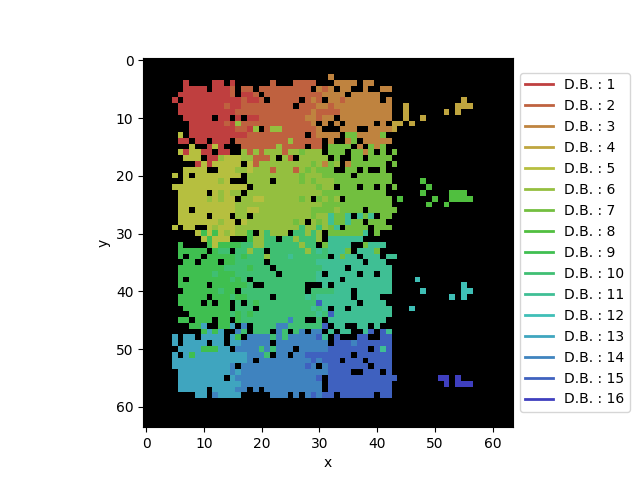
\includegraphics[scale=0.7]{Figures/visulization_prediction_4_n_neurons.png}
    \caption{Visualisation de l'emplacement des prédictions de chaque bloc de détection du modèle entraîné par la méthode de découpage de l'image pour le jeu de données "test" avec 16 blocs de détection (D.B.).}
    \label{fig:visulization_prediction_4_n_neurons}
\end{figure}

\begin{figure}[hbt!]
    \centering
    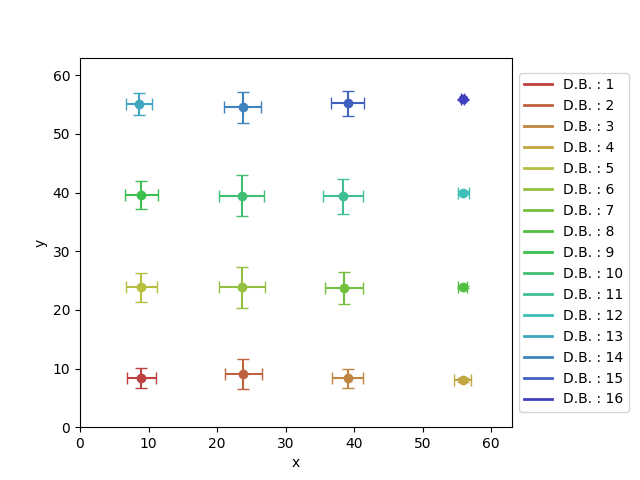
\includegraphics[scale=0.7]{Figures/visulization_prediction_4_n_neurons_mean_std.png}
    \caption{Visualisation de la moyenne et écart-type des prédictions de chaque bloc de détection du modèle entraîné par la méthode de découpage de l'image pour le jeu de données "test" avec 16 blocs de détection (D.B.).}
    \label{fig:visulization_prediction_4_n_neurons_mean_std}
\end{figure}

\break

\subsection{Évaluation du modèle}

L'évaluation de notre modèle est relativement similaire à celle réalisée pour YOLOv8 (\ref{subsec:yolov8_model_evaluation}). La principale différence réside dans la manière de calculer l'\acrshort{iou}. En effet, notre modèle ne nous retournant pas la largeur et la hauteur des boîtes de détection, nous définissons celle-ci manuellement aux mêmes valeurs que pour les labels de YOLOv8, c'est-à-dire à 5 pixels.

\subsection{Quantification du modèle avec QKeras}
\label{subsec:qkeras_quantization}

Dans l'optique de synthétiser notre modèle avec \acrshort{hls4ml}, nous avons utilisé la bibliothèque QKeras [\cite{noauthor_qkeras_2023}] afin de quantifier notre réseau de neurones. Cette approche consiste à réduire la précision des poids, activations, et gradients de notre réseau, afin de le rendre plus adapté à une implémentation sur \acrshort{fpga} où les ressources y sont limitées.

La quantification réalise une réduction du nombre de bits nécessaires pour représenter une valeur. Dans le cadre de ResNet18+Tête, cela aura pour effet de diminuer la précision des nombres, passant d'une représentation en virgule flottante à virgule fixe. Bien que cette diminution de précision puisse provoquer une baisse des performances, cette représentation étant similaire à celle des \acrshort{fpga}, les résultats obtenus devraient être similaires.

Lors de cette étape, nous avons uniquement modifié l'ensemble des couches de convolution, de Dense, de normalisation par lots, et d'activation par leurs versions quantifiées. Il est possible d'indiquer pour certaines de ces couches le nombre de bits à utiliser. Ainsi, nous avons décidé de travailler avec 16 bits, dont 6 sont utilisés pour représenter la partie entière.

Par ailleurs, la version quantifiée de la fonction d'activation sigmoïde propose soit une approximation assez pauvre, soit la possibilité d'utiliser la fonction définie par la librairie Keras. Étant donné que la qualité de cette fonction a un impact direct sur les performances de notre modèle, nous avons choisi d'utiliser la fonction définie par Keras.

\subsection{Synthétiser le modèle avec HLS4ML}
\label{subsec:r18_synthetize_with_hls4ml}

Afin de pouvoir implémenter notre modèle quantifié sur \acrshort{fpga}, nous devons d'abord le synthétiser à l'aide de \acrshort{hls4ml}. Lors de cette phase, nous nous sommes heurtés à plusieurs contraintes / limitations détaillées dans la section \ref{sec:hls4ml_limitations}.

En plus de ces dernières, les ressources nécessaires pour synthétiser un modèle avec \acrshort{hls4ml}, notamment la mémoire vive, dépendent de la taille de ce dernier. Même s'il est possible de modifier le "ReuseFactor" qui va indiquer combien de fois un élément peut être réutilisé, nous avons souhaité réaliser une synthèse de ResNet18+Tête avec un "ReuseFactor" de $1$, afin de minimiser la latence. C'est pourquoi nous travaillons pour cette partie sur une version de ResNet18 dont les filtres des convolutions ont été divisés par 16. Malgré cela, les dernières couches de convolution de notre modèle avec un kernel de $3 \times 3$ possèdent trop d'éléments, et ne peuvent malheureusement pas utiliser la stratégie "Latency", raison pour laquelle elles ont été définies à "Resource".

Il faut également prendre en compte que comme nous ne pouvions malheureusement pas réutiliser une variable dans notre modèle plus de trois fois, et étant donné que nous réutilisons la sortie de notre version raccourcie de ResNet18 deux fois dans chacun de nos blocs de détections, nous ne pouvons utiliser qu’un seul bloc pour la synthèse de notre modèle.

%----------------------------------------------------------------------------------------
